\subsection{Degrees of Freedom}
So there was something I neglected to explicitly tell you in the previous section\footnote{Hahahaha I'm so evil.}. Not all gases are ideal. In fact, most gases aren't ideal\footnote{Although most are almost ideal.}. Now's when I explain why this is. And to do that, I need to explain degrees of freedom.
\subsubsection{What are Degrees of Freedom?}
What a degree of freedom is can depend on the subject. For the purposes of thermodynamics, it's a way in which a particle can store energy. For example, the point-like particles that I talked about in ideal gas law can store energy in their motion along each directional axis. This gives them three degrees of freedom. That being said, there's a bunch of ways particles can store energy. They can vibrate, rotate, and have potential energy. The more of these a particle can do, the more degrees of freedom it has. However, not all degrees of freedom survive, because of reasons arising from quantum mechanics,\footnote{As you will learn next term, in quantum mechanics, energy is discretized (i.e. not continuous). If the amount of energy that could be stored in a potential degree of freedom is too small to get to the next discrete energy level, it'll be "frozen out". When that occurs, no energy can be stored in that way at all.} but essentially, each degree of freedom must store a minimum amount of energy to exist at all. 
\subsubsection{The Equipartition Theorem}
The equipartition theorem states that:
\begin{center}
    At thermal equilibrium, the thermal energy of a system is equally divided amongst all available degrees of freedom.
\end{center}
The equipartition theorem tells us that a a single quadratic degree of freedom \footnote{A quadratic degree of freedom is simply one where the energy goes by the square of some property; for example, the kinetic energy in the x direction is $E_{x} = \frac{1}{2}mv_x^2$, which is quadratic in the $v_x$ term.}, and therefore that one dimension of kinetic energy, has a magnitude of:
\begin{equation*}
    \epsilon_{k}=\frac{1}{2}{k_{b}}T.
\end{equation*}
 We also know that the total internal energy of the system is simply the sum of the energy of each particle. So
\begin{gather}
    E_{th}=\frac{\chi}{2}N{k_{b}}T \\
    E_{av}=\frac{\chi}{2}{k_{b}}T
\end{gather}
Here, $N$ represents the number of particles in the system, and $k_b$ is the Boltzmann constant, a fundamental constant of nature with a precisely defined value. $\chi$ is the number of degrees of freedom in a molecule, which happens to be $3$ for monotomic gases (corresponding to three translational degrees of freedom). A more comprehensive list is given in the section below. $T$ is temperature, in \textbf{Kelvin}. In questions 2 and 3 below, you will show that:
\begin{equation}
E_{th} = \frac{\chi}{2}nRT
\end{equation}
Where $n$ is the number of mols of gas, and $R$ is the gas constant ($R = 8.3145 \textrm{ J} \textrm{ mol}^{-1} \textrm{ K}^{-1}$). Now, we may define:
\[ c_v = \frac{\chi}{2}R \]
to be the specific heat capacity at a fixed volume. We now obtain the useful formula:
\begin{equation}
    E_{th} = nc_v T
\end{equation}
This formula is extremely useful for relating energy and temperature. Assuming that the amount and kind of gas you have doesn't change, this also allows us to look at the change in temperature and energy:
\begin{equation}
    \label{eqn:(13)}
    \Delta E_{th} = nc_v \Delta T
\end{equation}
The above formula will hold for any process where the amount of gas you have doesn't change, making it quite useful. It also has some immediately clear consequences. For one, it tells us that for a given amount of energy we give to a system, how much its temperature changes depends on two things; it depends on:
\begin{enumerate}
    \item The amount of stuff we have in the system, represented by the number of mols, $n$. This is fairly intuitive; the more stuff I have, the more energy I need to increase its temperature!
    \item The degrees of freedom of the molecules we are looking at. Imagine we were comparing two molecules, where one was simple molecule with few degrees of freedom (say, monotomic Helium), and a complex molecule with many degrees of freedom (say, a triatomic molecule), the former would have a lower heat capacity $c_v$ (check this from the definition!). Therefore, for a given amount of energy $\Delta E$ we give to a system, the system composed of molecules with fewer degrees of freedom will have a greater change in temperature (check this as well!). Physically, we might intuit this from the fact that molecules with a greater number of degrees of freedom have more degrees to which the energy can be distributed, and hence a smaller proportion of the energy goes into increasing the temperature. 
\end{enumerate}

Now, you may wonder why I have chosen to label $c_v$ the way I have (What do I mean by specific heat capacity at fixed volume?). This notation will soon become clear when we discuss the different thermodynamic processes. \\

Brief note before we move on; If you take the equipartition theorem to be a fundamental result\footnote{unfortunately, we will not be proving it here}, we obtain a derivation for our temperature definition in equation \ref{eqn:(8)} that works for any molecule (not just an ideal one). Any molecule in three dimensions would have three translational degrees of freedom, or three directions of kinetic energy. Therefore, the theorem would tell us that:
\[\epsilon_{kx}+\epsilon_{ky}+\epsilon_{kz} = \frac{1}{2}k_bT + \frac{1}{2}k_bT + \frac{1}{2}k_bT \]
So if we group the leftmost three terms into a general average kinetic energy term:
\[\epsilon_{kavg} = \frac{3}{2}k_bT \]
And rearranging for temperature:
\[T = \frac{2}{3k_b}\epsilon_{kavg} \]
So we have recovered our definition! In fact, you could combine this temperature definition with equation \ref{eqn:(2)} which we derived from first principles:
\[ \frac{3}{2} P V=N \epsilon_{kavg} \]
And actually derive the ideal gas law from scratch (without having to rely on it as an experimental result)!

\subsubsection{Degrees of Freedom of Different Molecule Types}
I've said that monoatomic, neutral gases have only three degrees of freedom. But as any good chemist knows\footnote{Don't confirm this with Chris or John} most elements don't like to be alone. So most gases aren't monoatomic. For example nitrogen gas, the most abundant gas in the atmosphere, is annoyingly diatomic. The ideal gas law doesn't apply to it (though, for reasonably low pressures\footnote{i.e. The range of pressures we would consider in Science One problems}, its behavior does not deviate far from an ideal gas, and we can apply the ideal gas law to it and be approximately correct. But the equation for energy does, if we could just figure out how many degrees of freedom it had, and the same is true for any gas. Anyways I'll stop prattling on now and tell you how many degrees of freedom these gases have (they're all kinetic degrees of freedom). \\
\newline
\begin{center}
\begin{tabular}{|c|c|c|}
    \hline
    Gas Type & \# of Deg of Freedom & Types of Deg of Freedom \\
    \hline
    Monoatomic & 3 & 3 translational \\
    \hline
    Diatomic & 5 & 3 translational, 2 rotational \\
    \hline
    Triatomic & 6 & 3 translational, 3 rotational \\
    \hline
\end{tabular}
\end{center}
\begin{figure}[h!]
    \centering
    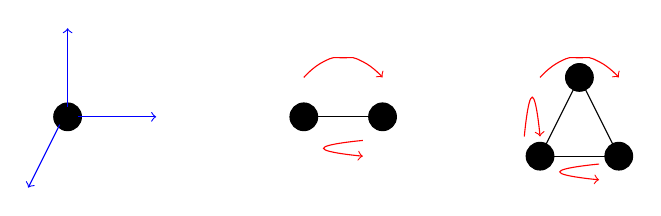
\begin{tikzpicture}
    \filldraw[fill=black, draw=black] (0,0) circle (5pt);
    \draw[->, blue] (0.13,0) -- (1.125,0);
    \draw[->, blue] (0,0.13) -- (0,1.125);
    \draw[->, blue] (-0.1,-0.1) -- (-0.5,-0.9);
    %\node[below] at (1,0) {$y$};
    %\node[left] at (0,1) {$z$};
    %\node[left] at (-0.5,-0.85) {$x$};
    
    \filldraw[fill=black, draw=black] (3,0) circle (5pt);
    \filldraw[fill=black, draw=black] (4,0) circle (5pt);
    \draw[black] (3,0) -- (4,0);
    \draw[->, red] plot [smooth, tension=1] coordinates {(3,0.5) (3.25,0.7) (3.5,0.75) (3.75,0.7) (4,0.5)};
    \draw[->, red] plot [smooth, tension=1] coordinates {(3.75,-0.3) (3.25,-0.4) (3.75,-0.5)};
    
    \filldraw[fill=black, draw=black] (6,-0.5) circle (5pt);
    \filldraw[fill=black, draw=black] (7,-0.5) circle (5pt);
    \filldraw[fill=black, draw=black] (6.5,0.5) circle (5pt);
    \draw[black] (6,-0.5) -- (7,-0.5);
    \draw[black] (6,-0.5) -- (6.5,0.5);
    \draw[black] (7,-0.5) -- (6.5,0.5);
    \draw[->, red] plot [smooth, tension=1] coordinates {(6,0.5) (6.25,0.7) (6.5,0.75) (6.75,0.7) (7,0.5)};
    \draw[->, red] plot [smooth, tension=1] coordinates {(6.75,-0.6) (6.25,-0.7) (6.75,-0.8)};
    \draw[->, red] plot [smooth, tension=1] coordinates {(5.8,-0.25) (5.9,0.25) (6,-0.25)};

    \end{tikzpicture}
    \caption{Visualization of the degrees of freedom of monoatomic, diatomic, and triatomic molecules. Monoatomic molecules only have three translational degrees of freedom, diatomic molecules have three translational plus two rotational degrees (it cannot rotate along the rotation axis parallel to its length), and the triatomic molecules have three translational and rotational degrees of freedom each.}
\end{figure}

\noindent
Liquids and solids have their own characteristic number of degrees of freedom too, I just didn't write them here. James/Chris might cover this in lecture however, so just because I didn't write it doesn't mean you don't need to know it\footnote{Really attach this disclaimer to the whole document}!
\newpage
\subsubsection{(Optional) Why Can't Monoatomic Molecules Rotate?}
After looking at that chart of degrees of freedom, you might be wondering: "Wait; why don't monoatomic gases have rotational degrees of freedom? What's stopping it from rotating?" The answer lies in the fact that the radius of atoms is extremely small; these leads to the atoms having a very small moment of inertia (you may recall that the moment of inertia of a sphere is $I = \frac{2}{5}MR^2$ where $M$ is the mass and $R$ the radius; if $R$ is small, then $R^2$ and therefore $I$ are extremely small). This has the consequence of the quantum energy levels of the rotational kinetic energy being extremely far apart. Hence these rotations are negligeble (i.e. not thermodynamically accessible) because they require a lot of energy to become excited; therefore, we do not consider the rotations as a degree of freedom\footnote{Since it's hard to get an intuition for why this is true, we can also consider a simpler (although oversimplified) explanation; if we approximate atoms as point particles of zero radius, then it becomes clear that they cannot rotate, and therefore the rotations cannot constitute a degree of freedom!}. You might be able to see why this argument generalizes to the diatomic molecule, as well (where you might have been wondering why it can't rotate along its length); the moment of inertia about the rotation axis along the length of the molecule is very small compared to the other two rotation axes; hence, rotations about that axis are not excited. 


